\documentclass[../main.tex]{subfiles}

\begin{document}

\justifying

\section{Ver energía potencial con tres partículas e interacción de dos cuerpos.}

\paragraph{Objetivo} Observar el registro de la energía potencial en un sistema de 3 partículas.

\subsection{Descripción de la simulación}

Se coloca una partícula en el centro de la caja de simulación, \(\vec{r}_2 = (0,0,0)\).
Se coloca una segunda partícula a una distancia de \num{0.75} de la partícula central, \(\vec{r}_1 = (-0.75,0,0)\).
Se coloca una tercera partícula a una distancia de \num{0.75} de la partícula centra, \(\vec{r}_3 = (0.75,0,0)\). 

Usando el comando \verb|fix move| se mueve la segunda partícula (\(\vec{r}_{1}\)) a velocidad constante de \num{0.1}, \(\vec{v}_2 = (0.1,0,0)\), hacia el centro de la caja.
Al mismo tiempo y usando el mismo comando, se mueve la tercera partícula a velocidad constante de \num{0.1}, \(\vec{v}_3 = (-0.1,0,0)\), hacia el centro de la caja.

El paso temporal es de \num{1d-3}.
El número de pasos es \num{4500}, obteniendo una simulación de \num{4.5} unidades temporales.

Cada interacción entre dos partículas, se le asigna el siguiente potencial
\begin{marginfigure}
    \centering
    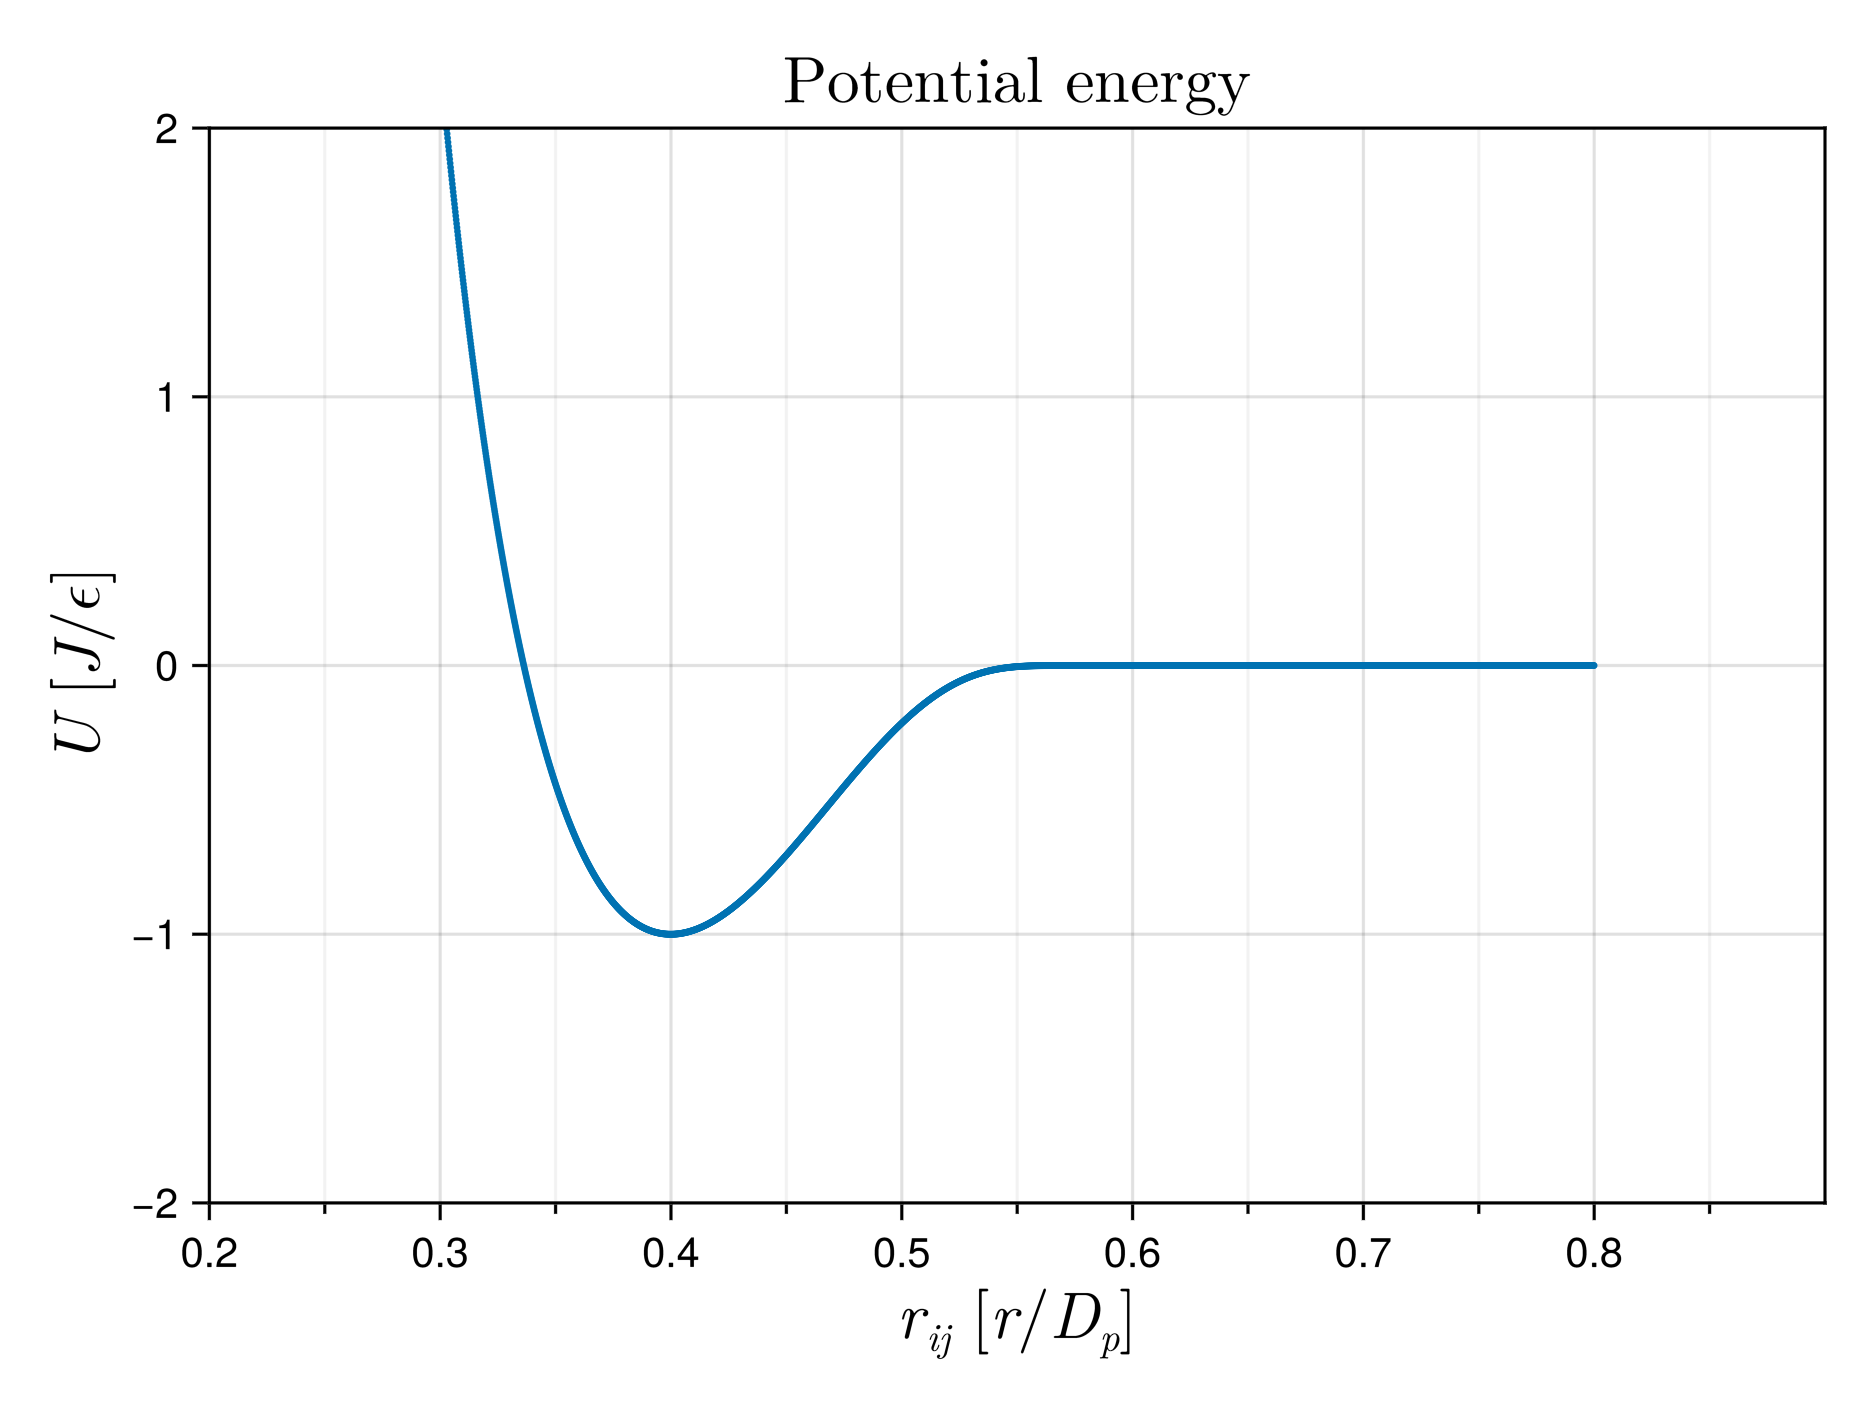
\includegraphics[width=0.8\textwidth]{../Figures/fig_Patchpot.png}
    \caption{Grafica del potencial de interacción entre \emph{patches}.
        \(\epsilon_{ij} = 1.0\), \( D_{p} = 0.4 \).
    }\label{fig:UpatchTeo}
\end{marginfigure}
\begin{gather}
    U_{\mathrm{patch}} = 
    \left\{
    \begin{array}{lc}
        2\epsilon_{ij}\left( \frac{1}{2}\left(\frac{D_p}{r_{ij}}\right)^{4}-1\right)\exp\left[\frac{D_{p}}{r_{ij}-r_{c}}+2\right]  & r_{ij}\in\qty[0,r_c] \\
        0 & r_{ij}>r_c
    \end{array}
    \right.\label{eqn:Upatch}
\end{gather}

La distancia entre los centros de las partícula está representada por \(r_{ij}\).
El parámetro \(\epsilon_{ij}\) controla el mínimo del potencial.
\(D_p\) es el diámtero de las partículas\footnote{La distancia entre los centros de las partículas esféricas.}.
El parámtero \(r_c\) es la distancia de corte definida en términos del diámetro de las partículas, \(r_c = 1.5 D_{p}\).

En el script de LAMMPS se registra la energía potencial con los siguientes comandos, \verb|compute ep all pe| y \verb|potAtom all pe/atom pair|.

\newpage

\section{Directory: 2026-02-11-102800}



\subsection{Resultados} En la figura~\ref{fig:Uatom1} se muestran 3 paneles.
Cada panel contiene la evolución temporal de la energía potencial registrada por \verb|pe/atom| y las distancias entre partículas $ij$ y $ik$.
En esta figura se puede observar que el mínimo del potencial registrado es \num{0.5} para la partículas que se encuentrán a los lados de la partícula central (\(\vec{r}_1,~\vec{r}_3\)), mientrás que el mínimo del potencial de la partícula central \(\vec{r}_2\) es igual a \num{1.0}.
Por otro lado, podemos observar que las contribuciones a la energía potencial solamente provienen de las distancias $d_{12}$ y $d_{13}$.
Esto es, porque el rango de la distancia $r_{13}$ es mayor a la distancia de corte, \(r_{13}\geq r_c\).

\begin{figure}[!ht]
    \centering
    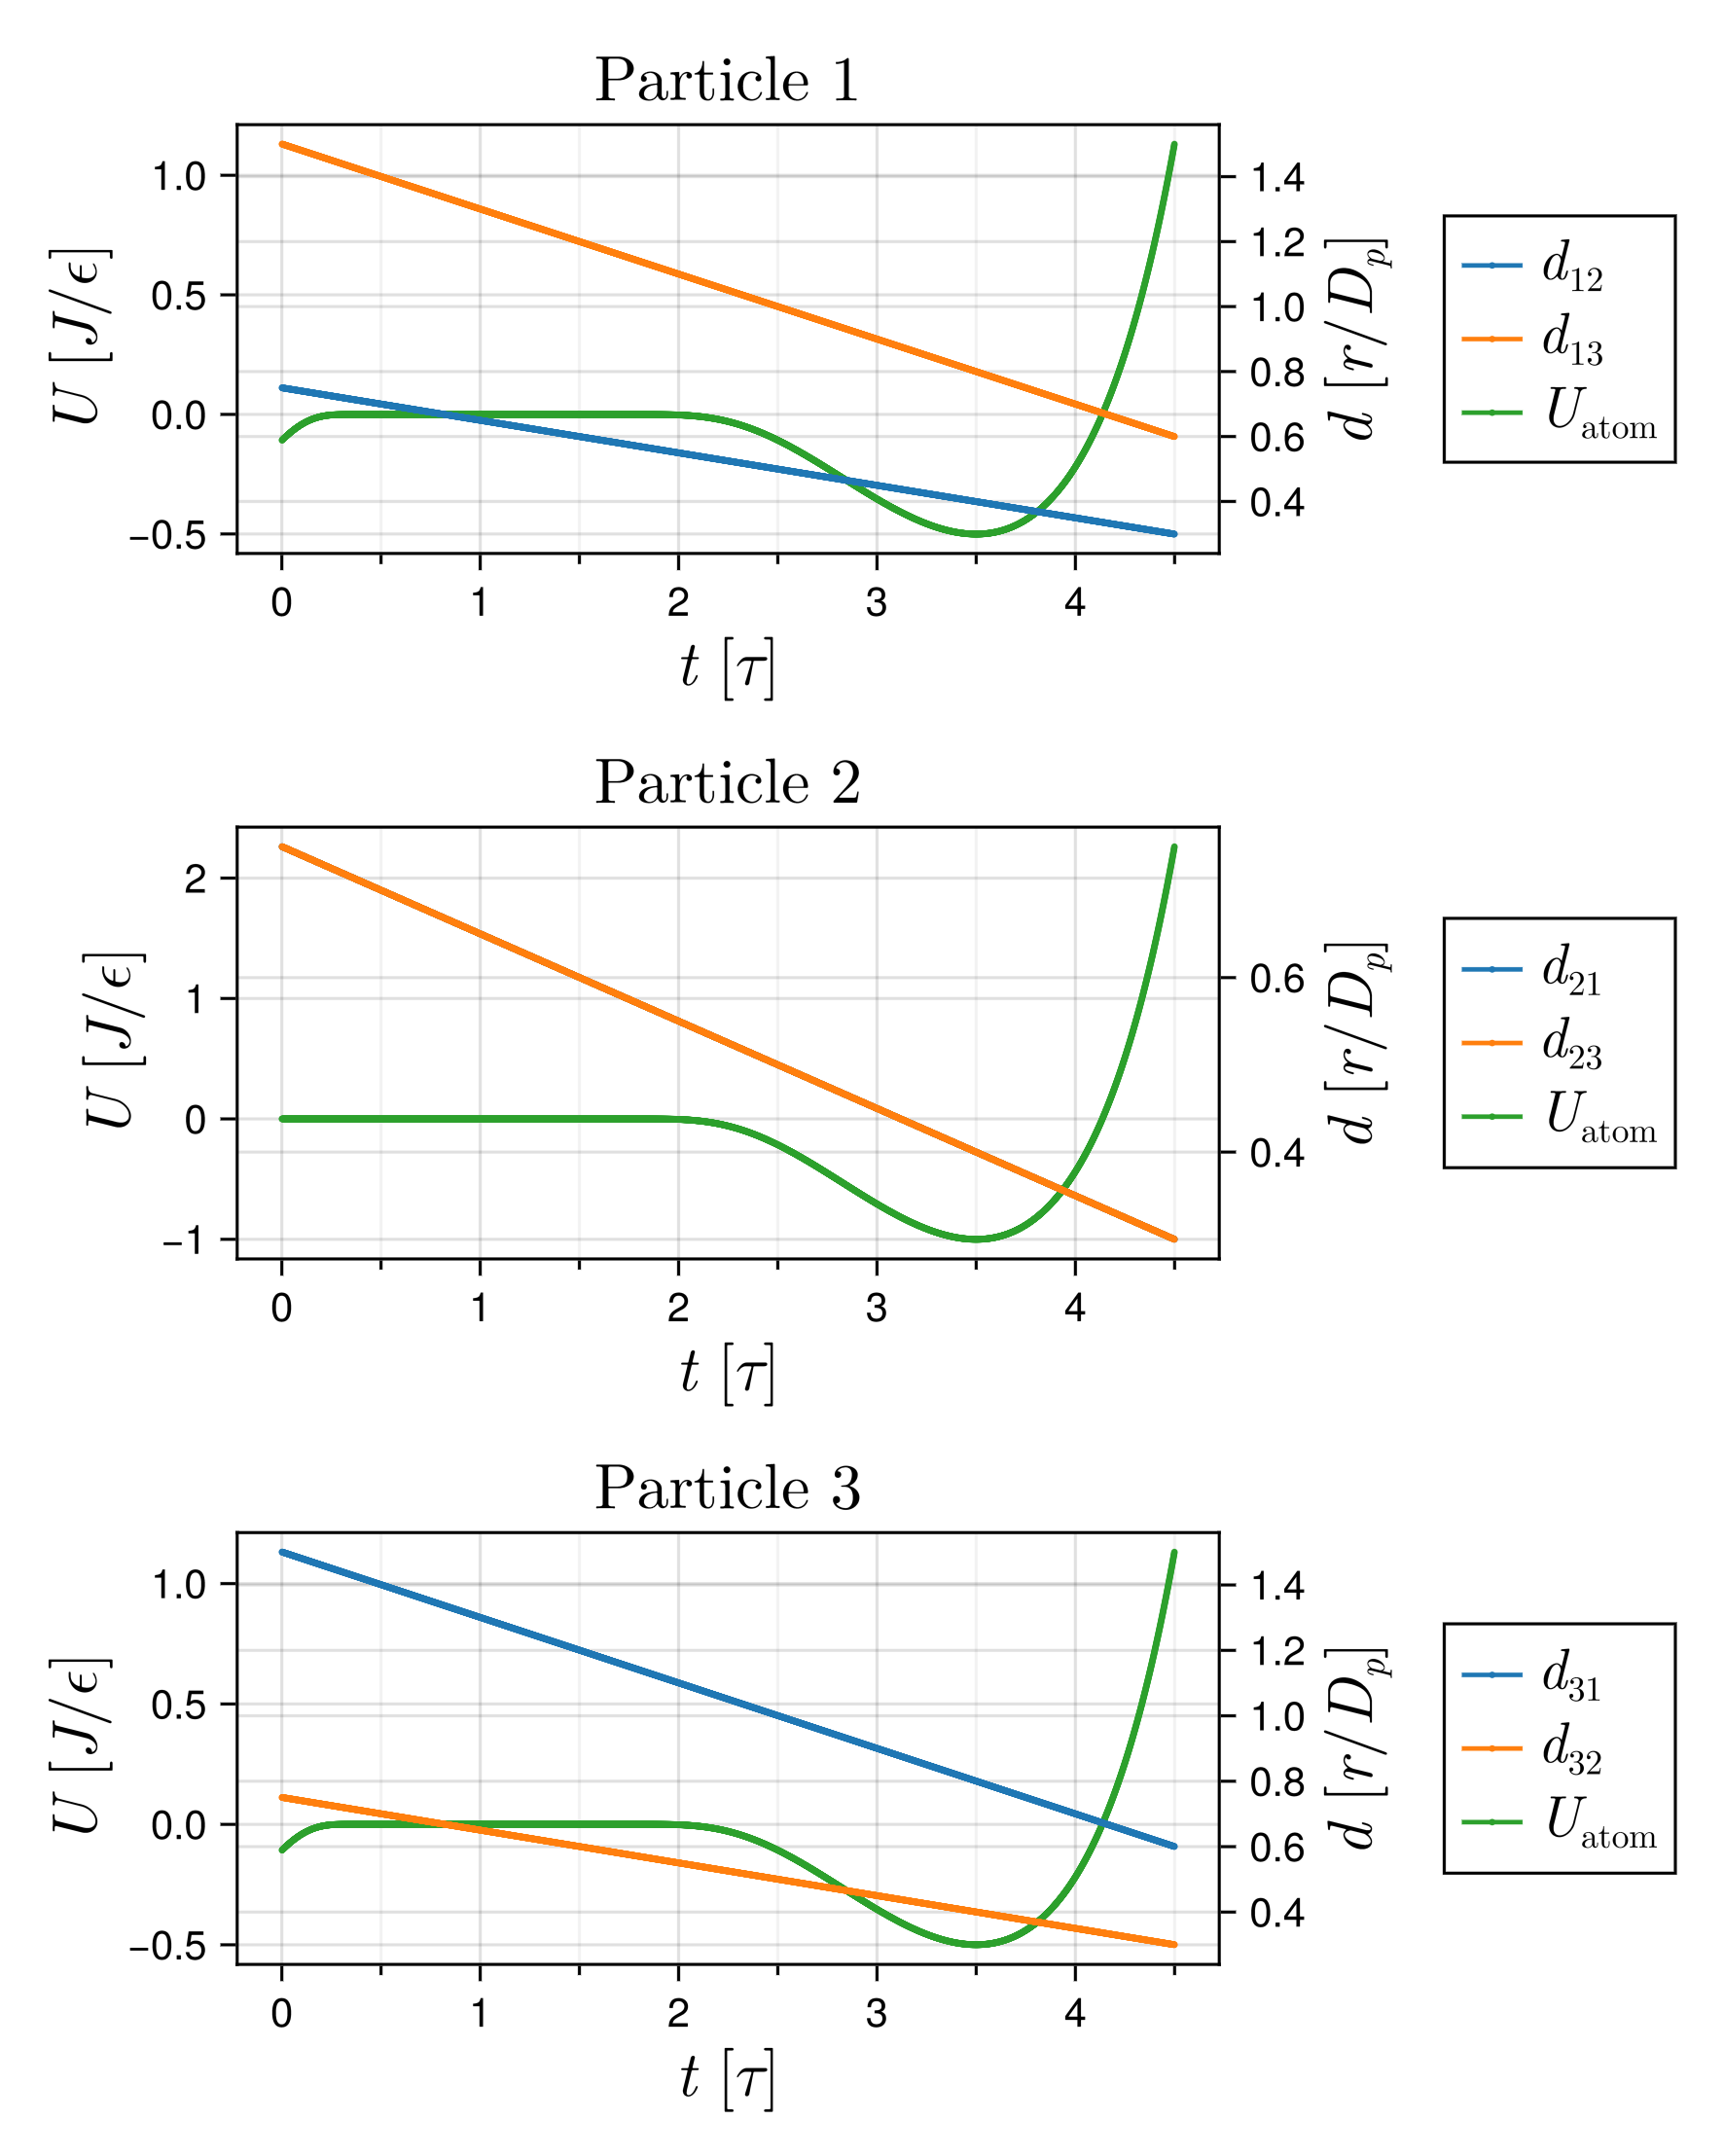
\includegraphics[width=0.8\textwidth]{../Figures/2026-02-11-102800/fig_Uatom.png}
    \caption{Energía potencial registrada por pe/atom.}\label{fig:Uatom1}
\end{figure}

\paragraph{Con respecto al mínimo del potencial registrado.}
Me esperaba observar un mínimo de potencial de \num{1.0} en las partículas \(\vec{r}_{1}\) y \(\vec{r}_3\), porque al evaluar las distancias entre esas partículas con la partícula central (\(\vec{r}_2\)), la función del potencial está tabulado para que el mínimo sea \num{1.0}.
Sin embargo, la partícula central la única que satisface la hipótesis.

Lo que interpreto de los resultados de la simulación, es que LAMMPS crea una \emph{normalización/interpolación}.
Esta normalización la puedo describir de la siguiente forma:
la partícula \(\vec{r_{1}}\) puede interactuar con las partículas \(\vec{r}_{2}\) y \(\vec{r}_3\).
Por definición del potencial, cada interacción tiene un mínimo de $\epsilon$.
Asumiendo que las distancias \(d_{1,2}\) y \(d_{1,3}\) son las que coincide con el mínimo del potencial, entonces la energía potencial de la partícula \(\vec{r}_{1}\) sería \(2\epsilon\).
Por lo tanto, para que la energía mínima del potencial de la partícula sea \num{1.0}, LAMMPS normaliza el potencial de tal forma que cada función potencial tenga un mínimo en \(\epsilon/N_{\mathrm{pi}}\).
En donde $N_{pi}$ es el número posible de interacciones con otras partículas usando ese mismo potencial.

Considerando lo anterior, eso es conscistente con los resultados obtenidos en la simulación.
Las partículas \(\vec{r}_{1}\) y \(\vec{r}_3\) solo tienen una interacción no nula, explicando el mínimo del potencial en \(\epsilon/2\) mientrás que la partícula \(\vec{r}_2\) está con dos interacciónes no nulas, explicando el mínimo de potencial en \(\epsilon\).

\paragraph{Acerca de la diferencia entre pe/atom y pe.}
Continuando con el análisis, también se analizó la energía potencial registrada por \verb|pe| y se comparó con las energías potenciales registradas por el comando \verb|pe/atom|.
Esa comparación se muestra en la figura~\ref{fig:Uatom-fix1}.
Además de la discusión anterior con respecto a la energía registrada por el comando \verb|pe/atom|, se puede observar que la suma de la energía potencial de cada partícula es el mismo resultado dado por el comando \verb|pe|.

\begin{figure}[!ht]
    \centering
    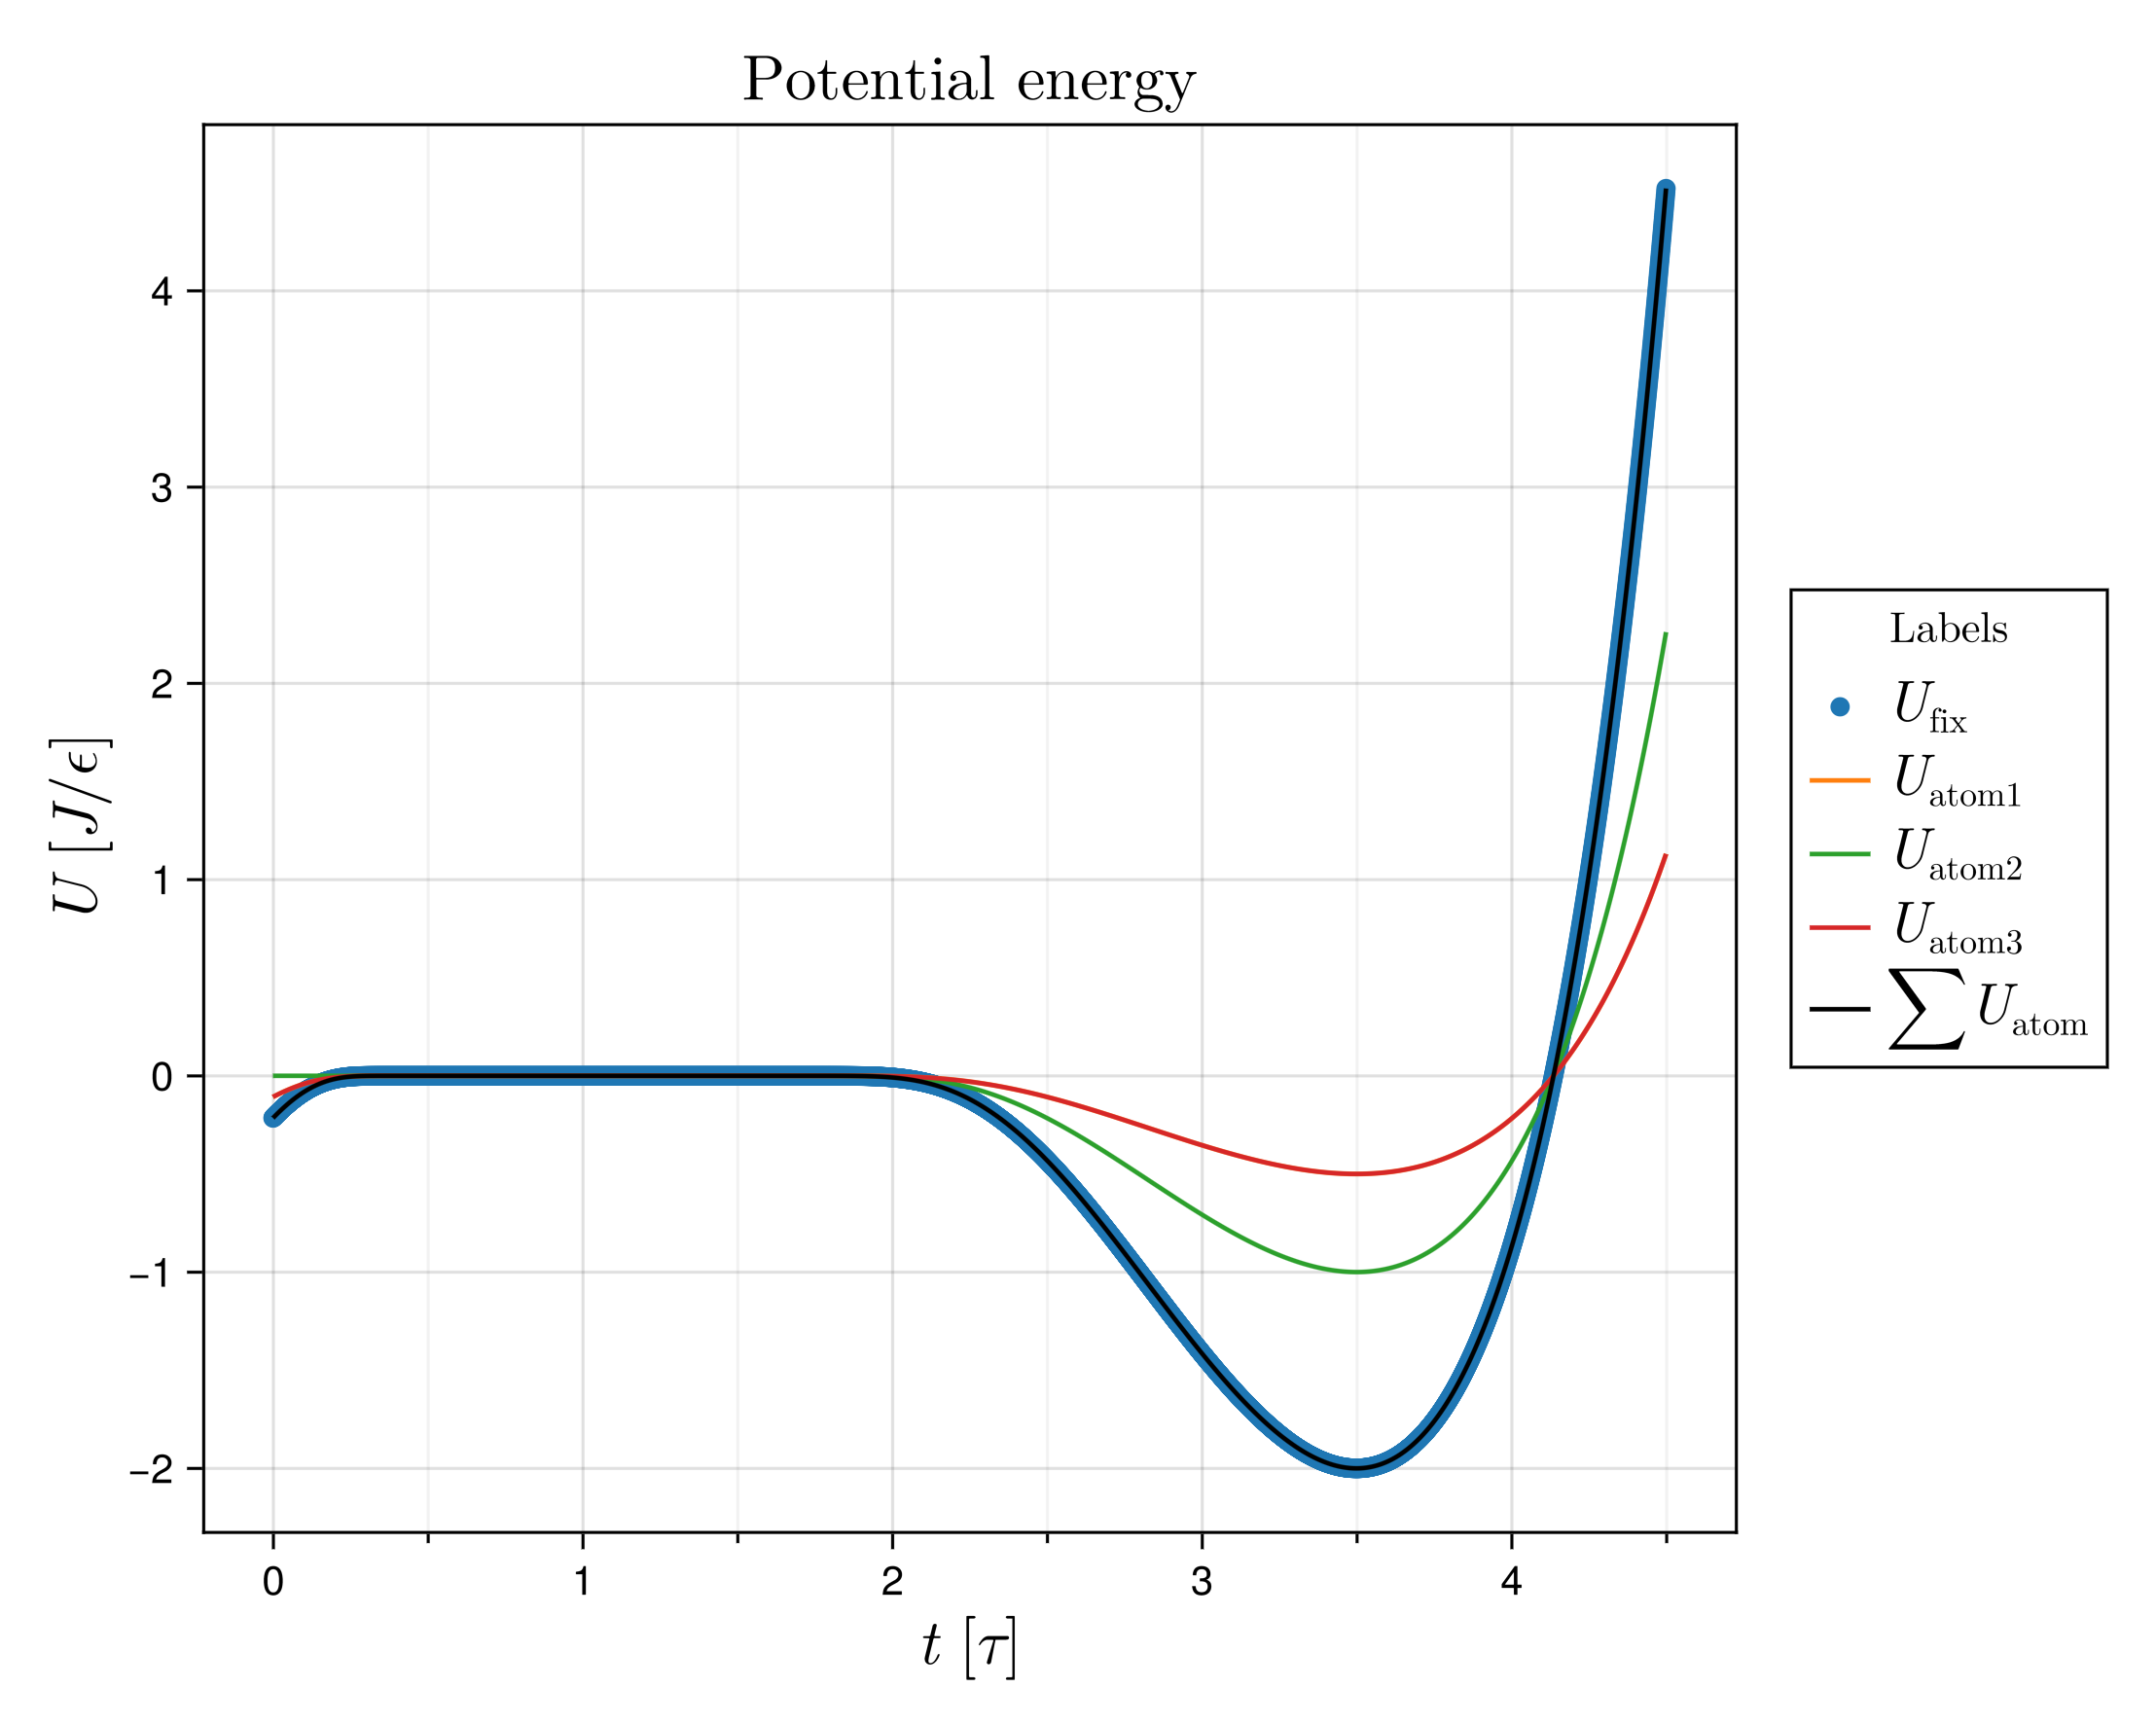
\includegraphics[width=0.8\textwidth]{../Figures/2026-02-11-102800/fig_Uatom-fix.png}
    \caption{ Comparación de la energía potencial registrada por pe/atom con la energía registrada por pe.
    }\label{fig:Uatom-fix1}
\end{figure}

El resultado dado por el comando \verb|pe| es esperado, porque hay dos distancias contribuyendo a la energía potencial, \(d_{1,2}\) y \(d_{2,3}\).
Cuando ambas distancias llegan al mínimo del pontencial, es sistema tiene un mínimo de \(2\epsilon\).
Agregando a la discusión, la \emph{normalización} que realiza LAMMPS para reportar la energía potencial en \verb|pe/atom| es conssistente con la energía potencial del sistema.

Por último, con la finalidad de asegurar que la energía reportada por el comando \verb|pe| es conscistente con la energía definida por la función~\eqref{eqn:Upatch}, se compara la energía reportada por ese comando con la energía dada por \(U_{\mathrm{patch}}\) evaluandola usando las distancias obtenidas en la simulación.
Esa comparación se muestra en la figura~\ref{fig:Ufix-func1}.

Al sumar las evaluaciones de la function \(U_{\mathrm{patch}}\) evaluada en las tres distancias, podemos observar que es igual a la energía potencial reportada por el comando \verb|pe|.
Eto permite usar la energía de \verb|pe| para encontrar errores con la energía potencial en futuras simulaciones.
También ayuda a observar que la energía de \verb|pe/atom| es equivalente a observar la energía por intreacción.

\begin{figure}[!ht]
    \centering
    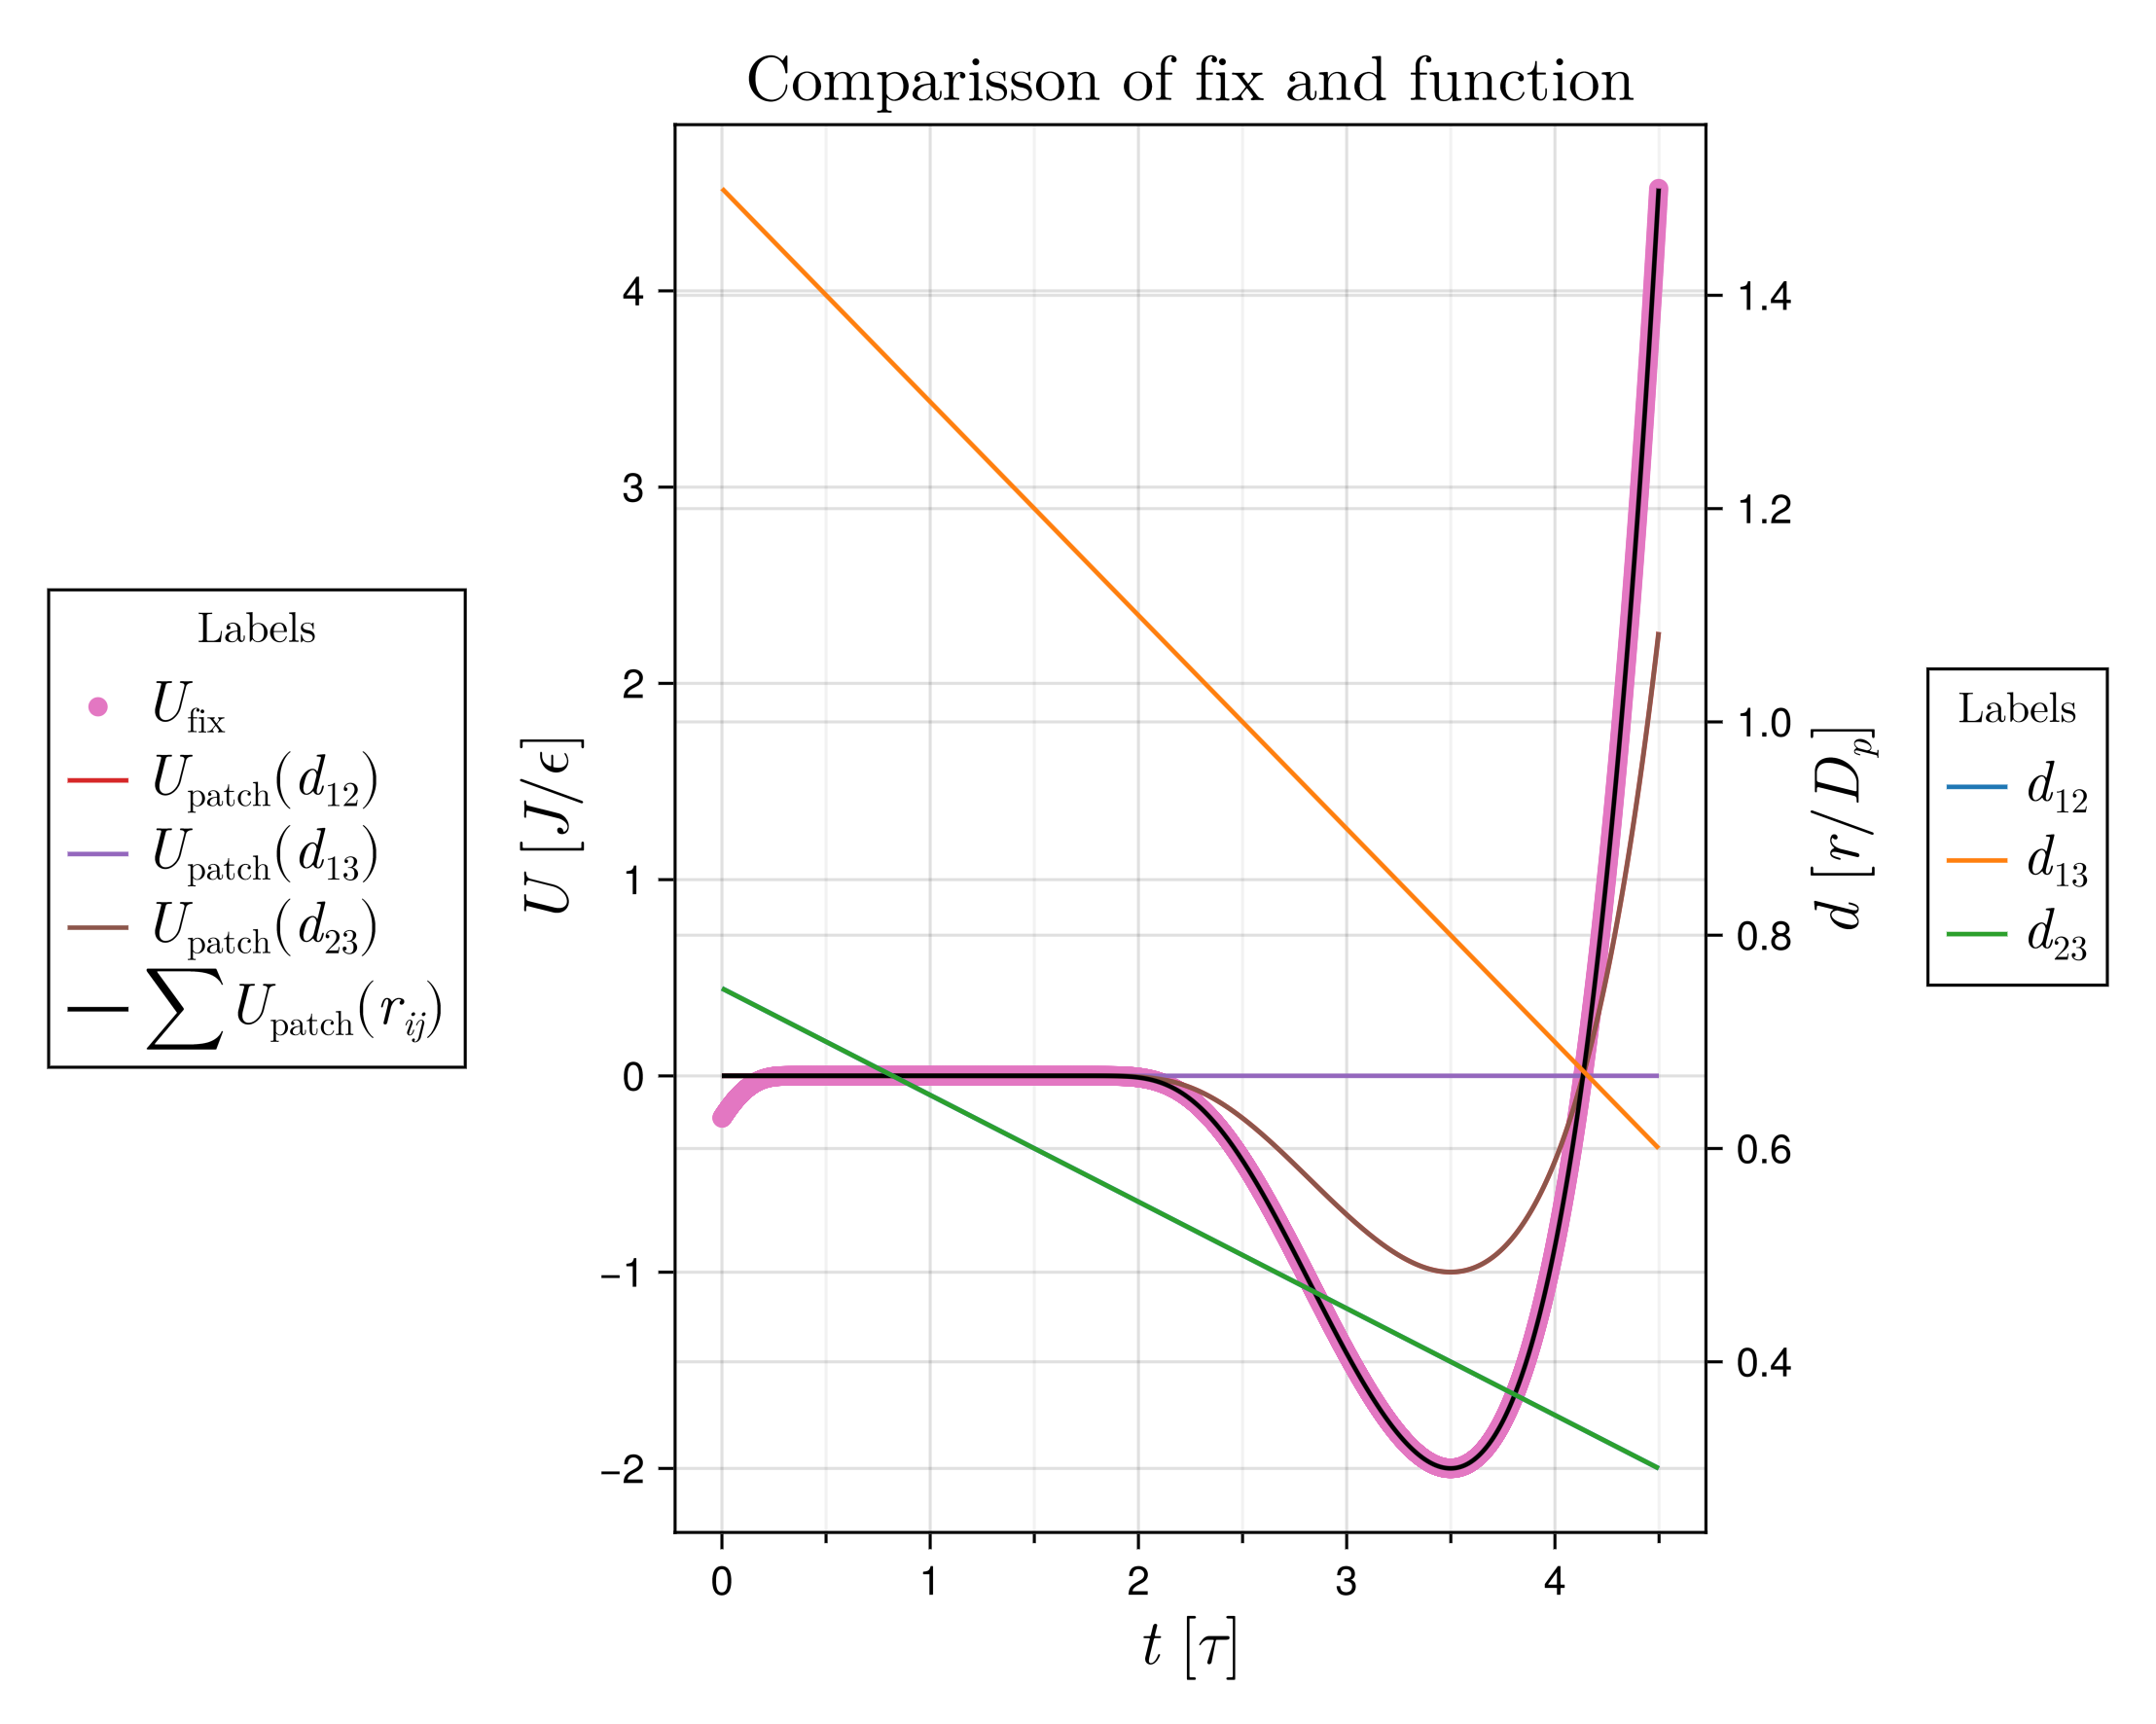
\includegraphics[width=0.8\textwidth]{../Figures/2026-02-11-102800/fig_Ufix-func.png}
    \caption{Comparación de la energía potencial registrada por pe con la energía potencial calculada usando las distancias de la simulación.
    }\label{fig:Ufix-func1}
\end{figure}

\paragraph{Acerca del potencial no nulo al inicio de la simulación.}
El motivo por el cuál se observa una contribución no nula al inicio de la simulación, es debido a que la simulación está declarada con condiciones de frontera peiódicas, ocasionando que \(d_{1,3}<r_c\), por lo tanto, se obtiene una contribución en la energía potencial.
Las posiciones iniciales de las partículas hacen que \(d_{1,3} = 0.5\) y al evaluar \(U_{\mathrm{patch}}(d_{1,3})=-0.21523723445950949\).
Al obtener el primer valor registrado por \verb|pe| obtenemos que es \num{-0.215238}, coincidiendo con la evaluación del potencial, confirmando que esa interacción no nula proviene de las condiciones de frontera periódicas.


\newpage

\subsection{Directory: 2026-02-11-125220}

\subsection{Descripción de la simulación}

Se coloca una partícula en el centro de la caja de simulación, \(\vec{r}_1 = (0,0,0)\).
Se coloca una segunda partícula en \(\vec{r}_2 = (-0.4,-0.4,0)\).
Se coloca una tercera partícula en \(\vec{r}_3 = (0.4,0.4,0)\). 

Usando el comando \verb|fix move| se mueve la segunda partícula a velocidad constante de \num{0.1}, \(\vec{v}_2 = (0.1,0,0)\), hacia el centro de la caja.
Al mismo tiempo y usando el mismo comando, se mueve la tercera partícula a velocidad constante de \num{0.1}, \(\vec{v}_3 = (-0.1,0,0)\), hacia el centro de la caja.

El paso temporal es de \num{1d-3}.
El número de pasos es \num{8000}, obteniendo una simulación de \num{8} unidades temporales.


\begin{figure}[!ht]
    \centering
    
\includegraphics[width=0.8\textwidth]{../Figures/2026-02-11-125220/fig_Uatom.png}
    \caption{Energía potencial registrada por pe/atom.}\label{fig:Uatom2}
\end{figure}




\begin{figure}[!ht]
    \centering
    
\includegraphics[width=0.8\textwidth]{../Figures/2026-02-11-125220/fig_Uatom-fix.png}
    \caption{ Comparación de la energía potencial registrada por pe/atom con la energía registrada por pe.
    }\label{fig:Uatom-fix2}
\end{figure}

\newpage

\begin{figure}[!ht]
    \centering
    
\includegraphics[width=0.8\textwidth]{../Figures/2026-02-11-125220/fig_Ufix-func.png}
    \caption{Comparación de la energía potencial registrada por pe con la energía potencial calculada usando las distancias de la simulación.
    }\label{fig:Ufix-func2}
\end{figure}


\newpage

\subsection{Directory: 2026-02-11-130434}

\subsection{Descripción de la simulación}

Se coloca una partícula en el centro de la caja de simulación, \(\vec{r}_1 = (0,0,0)\).
Se coloca una segunda partícula en \(\vec{r}_2 = (0.0,-0.4,0)\).
Se coloca una tercera partícula en \(\vec{r}_3 = (0.4,0.4,0)\). 

Usando el comando \verb|fix move| se mueve la tercera partícula a velocidad constante de \num{0.1}, \(\vec{v}_2 = (0.1,0,0)\), hacia el centro de la caja.

El paso temporal es de \num{1d-3}.
El número de pasos es \num{8000}, obteniendo una simulación de \num{8} unidades temporales.


\begin{figure}[!ht]
    \centering
    
\includegraphics[width=0.8\textwidth]{../Figures/2026-02-11-130434/fig_Uatom.png}
    \caption{Energía potencial registrada por pe/atom.}\label{fig:Uatom3}
\end{figure}




\begin{figure}[!ht]
    \centering
    
\includegraphics[width=0.8\textwidth]{../Figures/2026-02-11-130434/fig_Uatom-fix.png}
    \caption{ Comparación de la energía potencial registrada por pe/atom con la energía registrada por pe.
    }\label{fig:Uatom-fix3}
\end{figure}

\newpage

\begin{figure}[!ht]
    \centering
    
\includegraphics[width=0.8\textwidth]{../Figures/2026-02-11-130434/fig_Ufix-func.png}
    \caption{Comparación de la energía potencial registrada por pe con la energía potencial calculada usando las distancias de la simulación.
    }\label{fig:Ufix-func3}
\end{figure}





\end{document}
